%!TEX root = ../../../adrien_gomar_phd.tex

\subsection{Forced response}
\label{sub:forced_response}

As shown previously in Sec.~\ref{sec:cror_unsteady}, wakes and
potentials effects give rise to unsteady fluctuations in 
CROR configurations. These fluctuations 
can generate large vibration levels on the blades.
When the assembly modes are excited by the rotation speed
or its multiples, resonance can occur,
hence the term forced response. 
The frequency associated to the rotation speed or its multiples
is called Engine Order (EO).
At design, one step to minimize forced response is
to use the Campbell diagram shown in Figure~\ref{fig:campbell}
which schematically represents such resonance.
Blue points show the crossing of engine order with 
the blade eigen-frequencies within the operating range. 
The Campbell diagram does not give any information about
the absolute level of vibration. Therefore, it is mostly
used to rank potential designs~\cite{Marshall1996}. This phenomenon
will not be studied in this thesis.
\begin{figure}[htp]
  \centering
  \includegraphics*[width=0.40\textwidth]{campbell.pdf}
  \caption{Campbell diagram with forced response (blue circles)
  and flutter behavior (red stars).}
  \label{fig:campbell}
\end{figure}


\subsection{Flutter}
\label{sub:flutter}

Flutter is defined as a self-excited, unstable 
self-sustained vibration. In turbomachinery, this is
more likely to appear on blades.
One of the most impressive
manifestation of flutter occurred on the Tacoma Narrows
bridge in November 7\textsuperscript{th}, 1940.
Four months after being built, the bridge experienced 
torsional flutter excited by a 
\mbox{$64$~km.h\textsuperscript{-1}} wind.
The first and second torsional modes were observed.
A few hours later, the bridge felt down as seen in 
Figure~\ref{fig:tacoma_bridge}. Hopefully, no human
was injured, but this event showed the importance
of taking into account the flutter phenomenon as
it is a very energetic event and can lead to the failure of the system.
\begin{figure}[htp]
  \centering
  \subfigure[torsion mode]{
      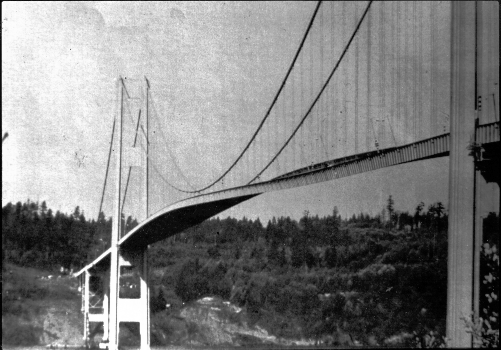
\includegraphics[height=.3\textwidth]{tac06.png}}
  \subfigure[failure of the bridge]{
      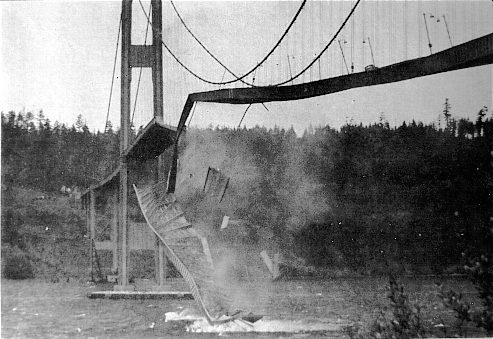
\includegraphics[height=.3\textwidth]{tac09.png}}
  \caption{Tacoma Narrows bridge flutter, from \citet{Smith1974}.}
  \label{fig:tacoma_bridge}
\end{figure}

Three vibration scenarios can appear, one leading to flutter.
The first scenario is the damped (or positively damped) 
vibration meaning
that the amplitude of the vibration decreases with respect to time, 
as shown in Figure~\ref{fig:flutter_damped}.
This is the most wanted behavior as the system tends to
a stable point. In this case, the blade is said to
be flutter-free for the studied mode.
The second scenario is the amplified (or negatively damped)
vibration, namely flutter, shown in Figure~\ref{fig:flutter_amplified}. 
This was the scenario that occurred on the Tacoma bridge. 
This scenario ultimately
leads to failure, which is not acceptable. This is particularly critical
on CROR configurations, as a blade failure might lead to 
the crash of the airplane as detailed in Sec.~\ref{sec:cror_challenges}.
The last scenario is the Limit Cycle Oscillation (LCO) vibration.
In this scenario, the deformation increases until a certain 
amplitude and then stays constant. This scenario is not
destructive by essence compared to the amplified scenario. However,
if the blade is repetitively excited by LCO, the blade
can fail because of structure fatigue.
\begin{figure}[htp]
  \centering
  \subfigure[damped (stable)]{
      \label{fig:flutter_damped}
      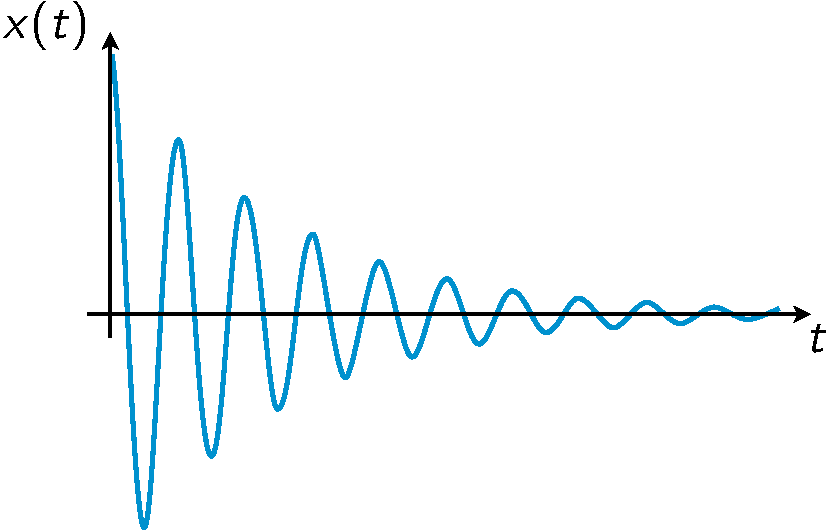
\includegraphics[width=.3\textwidth]{flutter_damped.pdf}}
  \subfigure[amplified (flutter)]{
      \label{fig:flutter_amplified}
      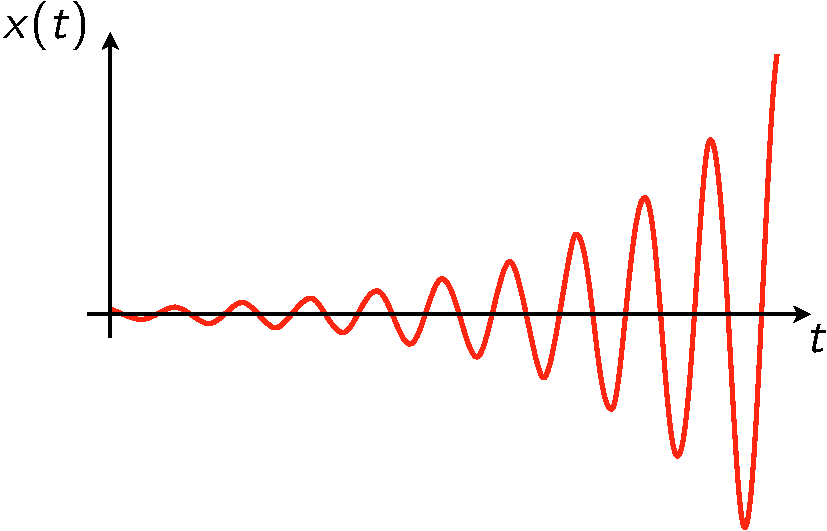
\includegraphics[width=.3\textwidth]{flutter_amplified.pdf}}
  \subfigure[limit cycle oscillation]{
      \label{fig:LCO}
      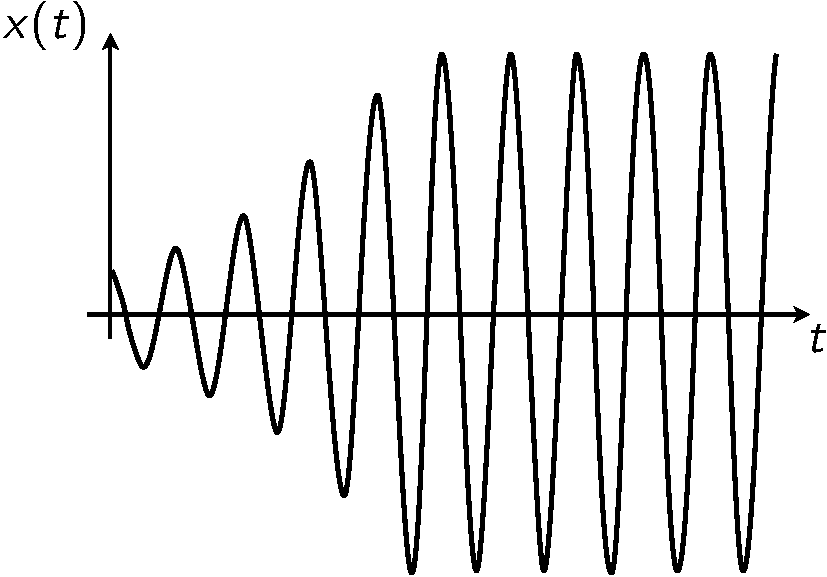
\includegraphics[width=.3\textwidth]{LCO.pdf}}
  \caption{Different vibration scenarios for the flutter phenomenon.}
\end{figure}

The development of one scenario over another one is linked to
the fluid response to the vibration of the blade. In fact,
if the aerodynamic loads projected on the direction of the displacement
is positive, this means that the vibration will be amplified. 
In opposite, if the force is in opposed direction, the vibration will be damped.
The out-of-phase component of the aerodynamic force compared to
the displacement vector will give finally the sign of the aerodynamic damping.
The amplitude will give its strength. 

In this thesis, only the flutter boundary is assessed
and a weak-coupling approach is chosen
as detailed in the following Section.
